\documentclass{article}
\usepackage[utf8]{inputenc}
\usepackage[spanish]{babel}

\title{Tarea 3}
\author{Rómulo Enrique Troncoso Pacheco}
\date{Septiembre 2020}

\usepackage{natbib}
\usepackage{graphicx}

\begin{document}


\maketitle

\section{Introducción}
El ploteo es una práctica comúnmente utilizada en revistas científicas, libros y materiales impresos, que sirven al lector para poder identificar de forma visual en forma de gráficas datos con mayor sencillez y comprensión en la exposición de elementos evaluados. Esto, genera la posibilidad de establecer estadísticas con fines comparativos relacionados a la identificación de cantidades  de letras y palabras que se puedan presentar en índices numéricos.

De esta forma, en esta práctica académica se establecen letras que mantienen una mayor frecuencia en el libro de The King in Yellow by Robert W. Chambers\cite{The_King_in_Yellow}, con la finalidad de generar un ejercicio de graficación de frecuencias en términos numéricos.
Con la finalidad de determinar una posible correlación entre las letras más frecuentes en el libro, se tomó como punto de referencia un diccionario con las palabras más frecuentes en inglés \cite{diccionario}. 

La importancia del ploteo es el establecer fundamentos para realizar un análisis de datos con la finalidad de emplearlo en diversas ramas de las ciencias. De esta forma, esta práctica se orienta a una serie de pasos en los cuales se ejecutaron de forma sistemática mediante instrucciones específicas incluyendo siete apartados donde se describe la secuencia a seguir para la utilización del lenguaje de programación utilizado R\cite{r}.

\section{Herramientas de desarrollo}
Dentro de la práctica se utilizaron lenguajes de programación, librerías y editores de textos que consistieron en:

Lenguaje de programación R\cite{r}: utilizado para el enfoque de análisis estadístico originado desde los cimientos del lenguaje S; cuya finalidad, era convertir ideas en software de forma rápida y fiel, por ello, se generaron las instrucciones que llevan una secuencia y lógica de pasos para cumplir algún objetivo en específico, como lo es el ploteo como instrucción.

Librerías: utilizado mediante un método de “librería” que consiste en fragmento de códigos, con el fin de facilitar las tareas al usuario para realizar una tarea en específico, para esta práctica se utilizaron las siguientes como gutenbergr\cite{gutenberg}, tidytext\cite{tidytext}, dplyr\cite{dplyr} y readr\cite{read}.

Editores de texto: utilizado el Visual studio code\cite{Visual_studio_code}, que ayuda a plantear el manejo del texto del scrip. 

\section{Metodología}
En la práctica se describen las letras con mayor impacto en el libro mencionado con antelación, con la finalidad de realizar una descripción exacta de los elementos, relacionado de forma sistemática de acuerdo a la técnica de filtrado que auxilió a concretar elementos exactos descriptivos en función a las letras del libro analizado. Aunado a ello, se analizó un total de 1000 palabras que son mayormente utilizadas en el idioma inglés, con el fin de comparar los resultados de frecuencia del libro con los resultados de frecuencia de las palabras del diccionario.

Para ello, se utilizó las gráficas de barras como herrramienta de ploteo que permitió establecer la altura de cada una, en función a la proporción de la frecuencia obtenida del elemento estudiado.

\section{Objetivo}
Representar gráficamente la frecuencia de letras en el libro The King in Yellow by Robert W. Chambers\cite{The_King_in_Yellow}.
Representar gráficamente la frecuencia de las letras de las palabras del diccionario.
\subsection{Objetivo específico}
Graficar letras filtradas relacionadas a la frecuencia del libro The King in Yellow by Robert W. Chambers\cite{The_King_in_Yellow}.
Graficar letras filtradas relacionadas a la frecuencia de las palabras del diccionario.
Comparar los resultados de los objetivos específicos previamente mencionados.
\section{Procedimiento}
Para poder llevar a cabo el objetivo planteado de la práctica fue necesario realizar lo siguiente de acuerdo a las herramientas mencionadas anteriormente:
\begin{itemize}
    \item Cargar el libro
    \item Separar letras
    \item Graficar letras filtradas
    \item Cargar diccionario
    \item Separar letras de las palabras
    \item Crear tabla de frecuencia de letras del diccionario
    \item Ordenar de forma decreciente las frecuencias
    \item Graficar las palabaras 
\end{itemize} 
\section{Conclusión}
\begin{enumerate}
    \item Se pudo graficar la frecuencia de las letras del libro analizado, referido en la sección de salida (Figura \ref{fig:letras}).
    \item Se pudo representar gráficamente la frecuencia de las letras de las palabras del diccionario (Figura \ref{fig:Letras_filtradas}).
    \item Se logró comparar los resultados de la gráfica de frecuencia del libro con la gráfica de frecuencia del diccionario.
    \item Se llegó a la conclusión de que las letras a, e, tuvieron un comportamiento similiar, puesto que en ambas gráficas aparecen como las letras con mayor frecuencia; por otra parte, las letras k, v, en ambos casos, fueron las que menor frecuencia tuvieron.
\end{enumerate}


\clearpage
\section{Salida}
En esta sección se muestran las salidas del sistema donde se incluyen las figuras \ref{fig:letras} y \ref{fig:Letras_filtradas}:
\begin{figure}[ht]
    \centering
    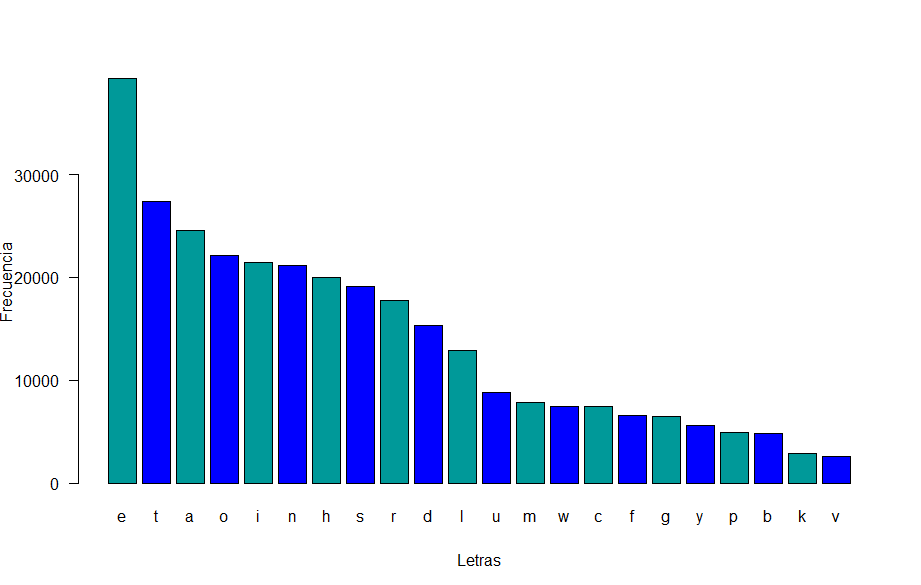
\includegraphics[scale=0.4]{Filtrado_letras_libro.png}
    \caption{En la figura se puede apreciar las letras con mayor frecuencia en libro analizado con una restricción de presentación a letras mayores a 1000 repeticiones.}
    \label{fig:letras}
\end{figure}
\begin{figure}[ht]
    \centering
    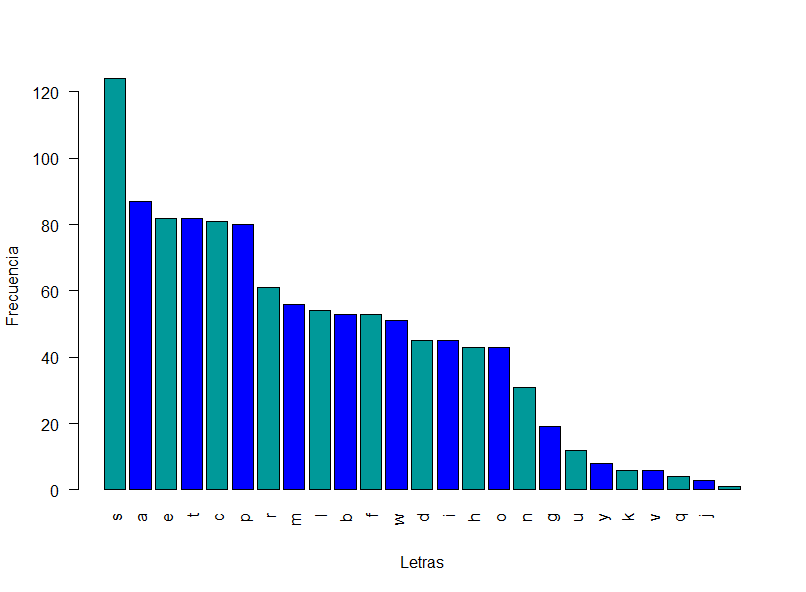
\includegraphics[scale=0.46]{Frecuencia_MU.png}
    \caption{En la figura se aprecia las letras con más repeticiones en el diccionario analizado con una restricción de búsqueda a las 1000 palabras con mayor frecuencia en el idioma inglés.}
    \label{fig:Letras_filtradas}
\end{figure}




\clearpage
\bibliographystyle{plain}
\bibliography{references}
\end{document}
